
\section{Grundlagen}

\subsection{Trivia}

Designer : Dennis Ritchie \newline
Erstveröffentlichung : 1972

\subsection{Rechnersystem system}

Grundaufbau eines Rechnersystem

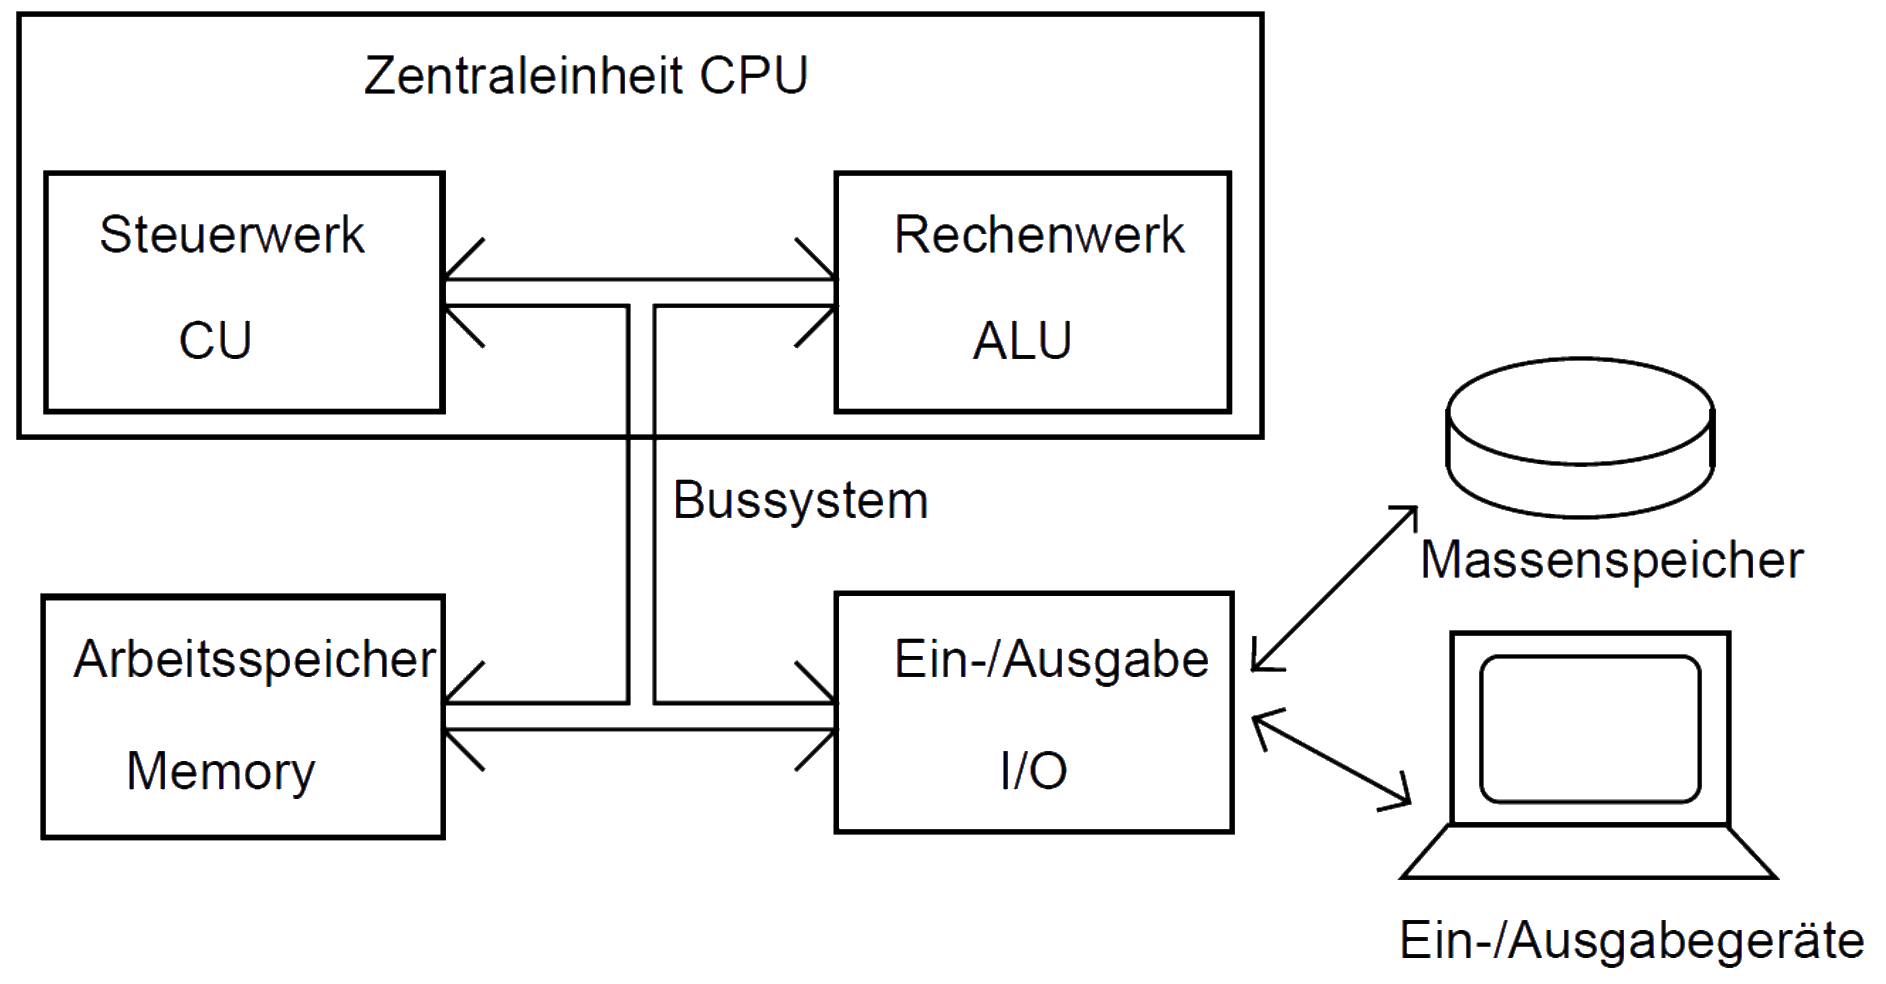
\includegraphics[width=1\columnwidth]{Pictures/PC_system_basicssystem.png}

\begin{center}
    \begin{tabular}{|c|c|c|} \hline  
        Grösse & Genauer Wert & näherungswert \\ \hline  
        Kilobyte & $2^{10}$ Bytes = 1024 Bytes & $10^3$ Bytes \\ \hline  
        Megabyte & $2^{20}$ Bytes = 1024 KB & $10^6$ Bytes \\ \hline  
        Gigabyte & $2^{30}$ Bytes = 1024 MB & $10^9$ Bytes \\ \hline 
    \end{tabular}
\end{center}

Die CPU kann $(2^{\text{Bitgrösse des Busses }} \cdot \text{ 8 bits})$ Ansteuern

\subsection{Zahlensysteme}

\subsubsection{Binär direkt}

Binär kann mittels 2er Potenz berechnet werden(geht auch bei Kommazahlen)\newline

\noindent
\begin{tabular}{|c|c|c|c|c|c|c|c|c|}
\hline
Gewichte: & \(2^7\) & \(2^6\) & \(2^5\) & \(2^4\) & \(2^3\) & \(2^2\) & \(2^1\) & \(2^0\) \\
\hline
Bitmuster: & 1 & 0 & 1 & 0 & 0 & 1 & 1 & 0 \\
\hline
\end{tabular}

\[
\begin{aligned}
Wert &= 1 \cdot 2^7+0 \cdot 2^6+1 \cdot 2^5+0 \cdot 2^4+0 \cdot 2^3+1 \cdot 2^2+1 \cdot 2^1+0 \cdot 2^0 \\
&= 128 + 0 + 32 + 0 + 0 + 4 + 2 + 0 \\
&= 166 \text{ (dezimal)}
\end{aligned}
\]

\subsubsection{Binär Zweierkomplement}

Das Zweierkomplement erlaubt das Darstellen von negativen Zahlen. Das MSB hat dabei den üblichen Wert negativ.\newline 
Um von Binär zum Zweierkomplement zu kommen, muss man alle Bits einer binär zahl invertieren und 1 addieren

\[
\overbrace{0110}^\text{6} 
\underbrace{\rightarrow}_\text{invert} 
\overbrace{1001}^\text{-7} 
\underbrace{\rightarrow}_{+1}
\overbrace{1010}^\text{-6} 
\]
\subsubsection{ASCII}

\textbf{A}merican \textbf{S}tandard \textbf{C}ode for \textbf{I}nformation \textbf{I}nterchange standardisiert die Repräsentation eines Bytes als Char. Da ASCII ein 7-bit Code ist, ist das MSB immer 0.

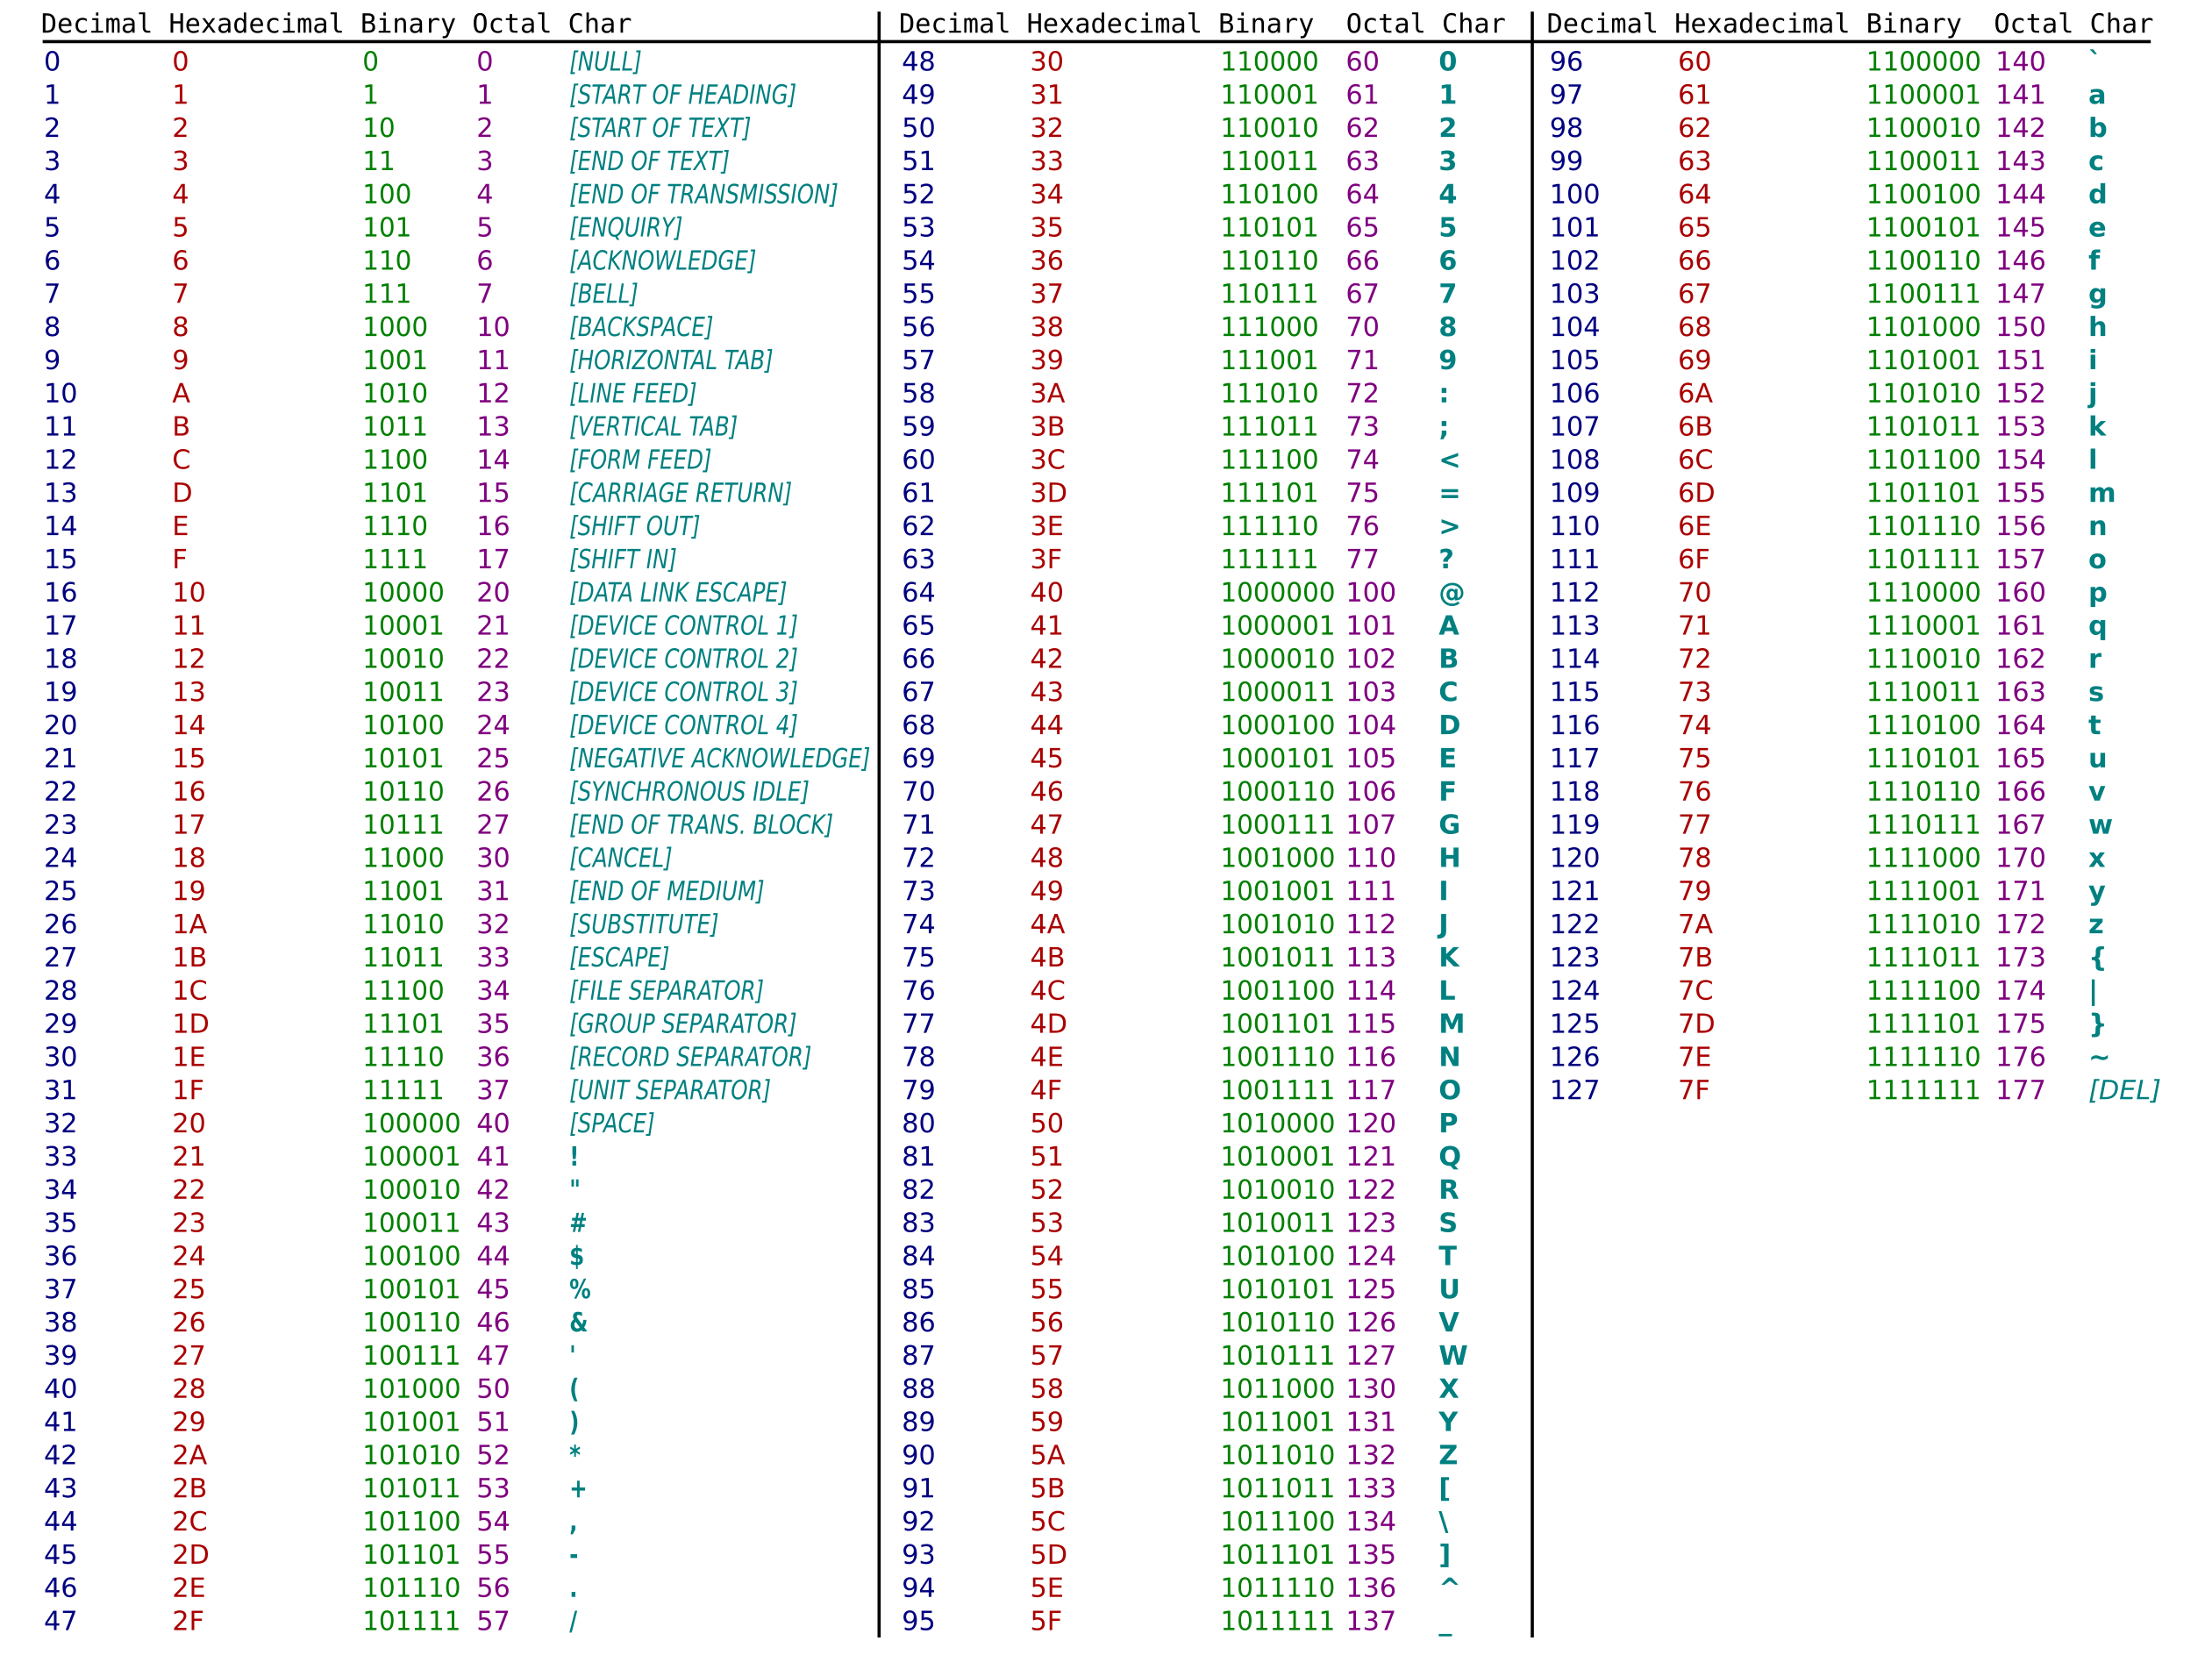
\includegraphics[width=1\columnwidth]{Pictures/ASCII_Table.png}

\subsubsection{Oktalzahlen}

Oktalzahlen erlauben nur 8 Ziffern (0 - 7). Als Bitmuster brauchen sie nur 3 Bits um 1 Ziffer darzustellen.
\[
\overbrace{110}^\text{6} 
\overbrace{001}^\text{1} 
\rightarrow 61
\]
Schreibweisen: $61_{\text{o}}$, $61_{\text{q}}$, $61_{\text{Oct}}$, 061\newline
Typischerweise mit 0 vor Beginn der Zahl.

\subsubsection{Hexadezimal}

Hexadezimal erlaubt 16 Ziffern(0-9,A-F). Binär stellen 4 Bits eine Hex Zahl dar.
\[
\overbrace{1100}^\text{A} 
\overbrace{0101}^\text{5} 
\rightarrow \text{0xA5}
\]

Schreibweisen: $\text{A5}_{\text{h}}$, A5H, $\text{A5}_{\text{hex}}$, $\text{A5}\$$, 0xA5\newline
Typischerweise mit 0x vor Beginn der Zahl.

\subsubsection{mrechnung beliebiges Zahlensystem zu dezimal}

Die jeweiligen Ziffern stellen jeweils ein Zahlenwert im System:\newline $n^0 \cdot x_1 + n^1 \cdot x_2 + n^2 \cdot x_3 + ....$ wobei n die Zahlenbasis ist.

\subsubsection{Umrechnung dezimal zu beliebigem Zahlensystem}

Die umzurechnende Zahl muss durch die Zahlenbasis mit Rest dividiert werden. Der Rest ist dann die erste Ziffer der entstehenden Zahl. Der erhaltene Quotient muss erneut dividiert werden und man erhält dann die folgenden Ziffern. Wenn der Quotient 0 erreicht hat, ist die Umrechnung fertig. 
